\documentclass[a4paper,10pt, notitlepage]{report}
\usepackage{geometry}
\geometry{verbose,tmargin=30mm,bmargin=25mm,lmargin=25mm,rmargin=25mm}
\usepackage[utf8]{inputenc}
\usepackage[sectionbib]{natbib}
\usepackage{amssymb}
\usepackage{amsmath}
\usepackage{enumitem}
\usepackage{xcolor}
\usepackage{cancel}
\usepackage{mathtools}
\usepackage{caption}
\usepackage{subcaption}
\usepackage{float}
\PassOptionsToPackage{hyphens}{url}\usepackage{hyperref}
\hypersetup{colorlinks=true,citecolor=blue}


\newtheorem{thm}{Theorem}
\newtheorem{lemma}[thm]{Lemma}
\newtheorem{proposition}[thm]{Proposition}
\newtheorem{remark}[thm]{Remark}
\newtheorem{defn}[thm]{Definition}

%%%%%%%%%%%%%%%%%%%% Notation stuff
\newcommand{\pr}{\operatorname{Pr}} %% probability
\newcommand{\vr}{\operatorname{Var}} %% variance
\newcommand{\rs}{X_1, X_2, \ldots, X_n} %%  random sample
\newcommand{\irs}{X_1, X_2, \ldots} %% infinite random sample
\newcommand{\rsd}{x_1, x_2, \ldots, x_n} %%  random sample, realised
\newcommand{\bX}{\boldsymbol{X}} %%  random sample, contracted form (bold)
\newcommand{\bx}{\boldsymbol{x}} %%  random sample, realised, contracted form (bold)
\newcommand{\bT}{\boldsymbol{T}} %%  Statistic, vector form (bold)
\newcommand{\bt}{\boldsymbol{t}} %%  Statistic, realised, vector form (bold)
\newcommand{\emv}{\hat{\theta}}
\DeclarePairedDelimiter\ceil{\lceil}{\rceil}
\DeclarePairedDelimiter\floor{\lfloor}{\rfloor}

% Title Page
\title{Exam 2 (A2)}
\author{Class: Bayesian Statistics \\ Instructor: Luiz Max Carvalho}
\date{02/06/2021}

\begin{document}
\maketitle

\textbf{Turn in date: until 16/06/2021 at 23:59h Brasilia Time.}

\begin{center}
\fbox{\fbox{\parbox{1.0\textwidth}{\textsf{
    \begin{itemize}
    \item Please read through the whole exam before starting to answer;
    \item State and prove all non-trivial mathematical results necessary to substantiate your arguments;
    \item Do not forget to add appropriate scholarly references~\textit{at the end} of the document;
    \item Mathematical expressions also receive punctuation;
    \item You can write your answer to a question as a point-by-point response or in ``essay'' form, your call;
    \item Please hand in a single, \textbf{typeset} ( \LaTeX) PDF file as your final main document.
 Code appendices are welcome,~\textit{in addition} to the main PDF document.
    \item You may consult any sources, provided you cite \textbf{ALL} of your sources (books, papers, blog posts, videos);
    \item You may use symbolic algebra programs such as Sympy or Wolfram Alpha to help you get through the hairier calculations, provided you cite the tools you have used.
    \item The exam is worth 100 %$\min\left\{\text{your\:score}, 100\right\}$
    marks.
    \end{itemize}}
}}}
\end{center}
% \newpage
% \section*{Hints}
% \begin{itemize}
%  \item a
%  \item b
% \end{itemize}
% 
\newpage

\section*{Background}

This exam covers applications, namely estimation, prior sensitivity and prediction.
You will need a working knowledge of basic computing tools, and knowledge of MCMC is highly valuable.
Chapter 6 in \cite{Robert2007} gives an overview of computational techniques for Bayesian statistics.

\section*{Inferring population sizes -- theory}

Consider the model
\begin{equation*}
 x_i \sim \operatorname{Binomial}(N, \theta),
\end{equation*}
with \textbf{both} $N$ and $\theta$ unknown and suppose one observes $\boldsymbol{x} = \{x_1, x_2, \ldots, x_K\}$.
Here, we will write $\xi = (N, \theta)$.

\begin{enumerate}[label=\alph*)]
 \item (10 marks) Formulate a hierarchical prior ($\pi_1$) for $N$, i.e., elicit $F$ such that $N \mid \alpha \sim F(\alpha)$ and $\alpha  \sim \Pi_A$.
 Justify your choice; 
 \item (5 marks) Using the prior from the previous item, write out the full joint posterior kernel for all unknown quantities in the model, $p(\xi \mid \boldsymbol{x})$. \textit{Hint:} do not forget to include the appropriate indicator functions!;
 \item (5 marks) Is your model identifiable?
 \item (5 marks) Exhibit the marginal posterior density for $N$, $p_1(N \mid \boldsymbol{x})$;
 \item (5 marks) Return to point (a) above and consider an alternative, uninformative prior structure for $\xi$, $\pi_2$.
 Then, derive $p_2(N \mid \boldsymbol{x})$;
 \item (10 marks) Formulate a third prior structure on $\xi$, $\pi_3$, that allows for the closed-form marginalisation over the hyperparameters $\alpha$ -- see (a) -- and write out $p_3(N \mid \boldsymbol{x})$;
 \item (10 marks) Show whether each of the marginal posteriors considered is proper.
 Then, derive the posterior predictive distribution, $g_i(\tilde{x} \mid \boldsymbol{x})$, for each of the posteriors considered ($i = 1, 2, 3$).
 \item (5 marks) Consider the loss function
 \begin{equation}
 \label{eq:relative_loss}
  L(\delta(\boldsymbol{x}), N) = \left(\frac{\delta(\boldsymbol{x})-N}{N} \right)^2.
 \end{equation}
 Derive the Bayes estimator under this loss.
\end{enumerate}

\section*{Inferring population sizes -- practice}
Consider the problem of inferring the population sizes of major herbivores~\citep{Carroll1985}.
In the first case, one is interested in estimating the number of impala (\textit{Aepyceros melampus}) herds in the Kruger National Park, in northeastern South Africa.
In an initial survey collected the following numbers of herds: $\boldsymbol{x}_{\text{impala}} = \{15, 20, 21, 23, 26\}$.
Another scientific question is the number of individual waterbuck (\textit{Kobus ellipsiprymnus}) in the same park.
The observed numbers of waterbuck in separate sightings were $\boldsymbol{x}_{\text{waterbuck}} = \{53, 57, 66, 67, 72\}$ and may be regarded (for simplicity) as independent and identically distributed.

\begin{figure}[H]
     \centering
     \begin{subfigure}[b]{0.45\textwidth}
         \centering
         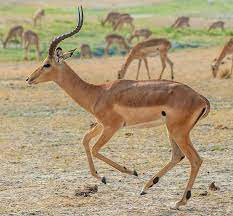
\includegraphics[scale=0.75]{figures/impala.jpeg}
         \caption{Impala}
     \end{subfigure}
     \begin{subfigure}[b]{0.45\textwidth}
         \centering
         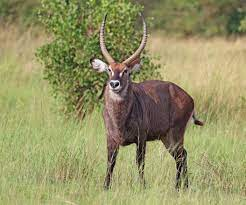
\includegraphics[scale=0.75]{figures/waterbuck.jpeg}
         \caption{Waterbuck}
     \end{subfigure}
        \caption{Two antelope species whose population sizes we want to estimate.}
        \label{fig:antelopes}
\end{figure}


\begin{enumerate}[label=\alph*)]
\setcounter{enumi}{8}
 \item (20 marks) For each data set, sketch the marginal posterior distributions $p_1(N \mid \boldsymbol{x})$, $p_2(N \mid \boldsymbol{x})$ and $p_3(N \mid \boldsymbol{x})$.
 Moreover, under each posterior,  provide (i) the Bayes estimator under quadratic loss and under the loss in (\ref{eq:relative_loss}) and (ii) a 95\% credibility interval for $N$.
 Discuss the differences and similarities between these distributions and estimates: do the prior modelling choices substantially impact the final inferences? If so, how?
 \item (25 marks) Let $\bar{x} = K^{-1}\sum_{k =1}^K x_k$ and $s^2 = K^{-1}\sum_{k =1}^K (x_k-\bar{x})^2$.
 For this problem, a sample is said to be \textit{stable} if $\bar{x}/s^2 \geq (\sqrt{2} + 1)/\sqrt{2}$ and \textit{unstable} otherwise.
 Devise a simple method of moments estimator (MME) for $N$.
 Then, using a Monte Carlo simulation, compare the MME to the three Bayes estimators under quadratic loss (\ref{eq:relative_loss}) in terms of relative mean squared error. 
 How do the Bayes estimators compare to MME in terms of the statibility of the generated samples? 
 \textit{Hint}: You may want to follow the simulation setup of~\cite{Carroll1985}. 
\end{enumerate}

\bibliographystyle{apalike}
\bibliography{a2}
\end{document}          
